%% USPSC-Introducao.tex

% ----------------------------------------------------------
% Introdução (exemplo de capítulo sem numeração, mas presente no Sumário)
% ----------------------------------------------------------
\chapter[Revisão Bibliográfica]{Revisão Bibliográfica}
\label{Revisão}
Neste capítulo, serão apresentadas as fundamentações teóricas das técnicas de aprendizado de máquina utilizadas neste trabalho juntamente com um levantamento de estudos correlatos na área da saúde que empregaram técnicas semelhantes.

\section{Aprendizado de Máquina}
A crescente complexidade nos desafios computacionais e o volume massivo de dados gerados por diversas fontes impulsionaram a necessidade de ferramentas computacionais mais avançadas. Neste contexto, o aprendizado de máquina define-se como um campo de estudo da IA que dá aos computadores a habilidade de aprender sem serem explicitamente programados. Para tal, no aprendizado de máquina, os computadores são treinados para aprender com dados passados, utilizando técnicas que os possibilitem a derivar uma função ou hipótese capaz de solucionar problemas a partir de observações específicas, oferecendo soluções baseadas em dados históricos \cite{faceli}.

Os sistemas de aprendizado de máquina podem seguir vários paradigmas de aprendizado. Existem sistemas supervisionados, não supervisionados, semi-supervisionados, auto-supervisionados e de reforço. O aprendizado supervisionado é usado quando o modelo pode ser treinado com exemplos rotulados, enquanto o aprendizado não supervisionado é usado quando não há rótulos disponíveis. O aprendizado semi-supervisionado é uma combinação dos dois, enquanto o auto-supervisionado é usado quando o modelo pode ser treinado com exemplos gerados automaticamente. O aprendizado por reforço é usado quando o modelo pode aprender a tomar decisões com base em recompensas e punições \cite{geron2022hands}.

Dentro do paradigma de aprendizado supervisionado, os algoritmos podem ser usados em tarefas de classificação ou regressão. A classificação é usada para prever classes, enquanto a regressão é usada para prever valores. Por exemplo, a classificação pode ser usada para prever se um e-mail é spam ou não, enquanto a regressão pode ser usada para prever o preço de uma casa com base em suas características \cite{geron2022hands}.

A seguir será apresentada uma breve introdução aos modelos de classificação utilizados no desenvolvimento deste projeto.

\subsection{K-Vizinhos Mais Próximos}

O algoritmo K-Vizinhos Mais Próximos (ou KNN, do inglês \textit{K-Nearest Neighbors}) é um método de classificação que opera com base na proximidade dos vizinhos mais próximos de um ponto de dados. Quando um novo ponto de dados precisa ser classificado, o algoritmo encontra os \textit{k} pontos mais próximos a ele a partir do conjunto de dados de treinamento. Em seguida, ele classifica o novo ponto de dados com base na classe mais frequente entre esses \textit{k} vizinhos mais próximos.
O algoritmo KNN assume que todas as observações correspondem a pontos em um espaço n-dimensional e não requer um processo de aprendizado. Ele apenas prevê a categoria do novo ponto de dados com base nas categorias dos pontos conhecidos no momento da classificação \cite{Wang_2019}.

Os “vizinhos mais próximos” de uma instância são mensurados por métricas de distância, tais como a distância Euclidiana ou de Manhattan. A título de exemplo, será apresentada a distância Euclidiana, definida pela \autoref{eq:dist}:

\begin{equation}
\label{eq:dist}
    d(x, x') = \sqrt{\sum_{i=1}^{n} (x_i - x_i')^2}.
\end{equation}

\subsection{Regress\~ao Logística}

A regressão logística é um modelo estatístico usado para modelar a probabilidade de um evento ocorrer em termos de variáveis independentes \cite{logreg}. O modelo logístico é baseado na função logística, definida pela \autoref{eq:logreg}. Na \autoref{img:logreg}, é apresentado um exemplo da curva logística.

\begin{equation}
    \label{eq:logreg}
    f(z) = \frac{1}{1 + e^z}.
\end{equation}

De forma simplificada, o modelo logístico pode ser definido da seguinte maneira:

\begin{equation}
    \hat{y} = f(Z) = P(y = 1 | Z) = \frac{1}{1 + e^{-Z}}.
\end{equation}

onde $P(y = 1 | Z)$ é a probabilidade de ocorrência da classe positiva dado Z. Sendo Z:

\begin{equation}
    Z = \ln(\frac{p}{1 - p}) = \alpha + \sum_{j=1}^{k} \beta_k X_{ik}.
\end{equation}

onde \textit{p} representa a probabilidade de ocorrência do evento de interesse, enquanto \textit{X} denota o conjunto de variáveis preditoras. Os parâmetros do modelo, $\alpha$ e $\beta$, são estimados por meio da técnica de máxima verossimilhança \cite{favero}. Essa abordagem visa encontrar uma combinação de coeficientes que maximize a probabilidade de ocorrência do evento de interesse.

\begin{figure}
    \centering
    \caption{\label{img:logreg}Exemplo de função logística.}
    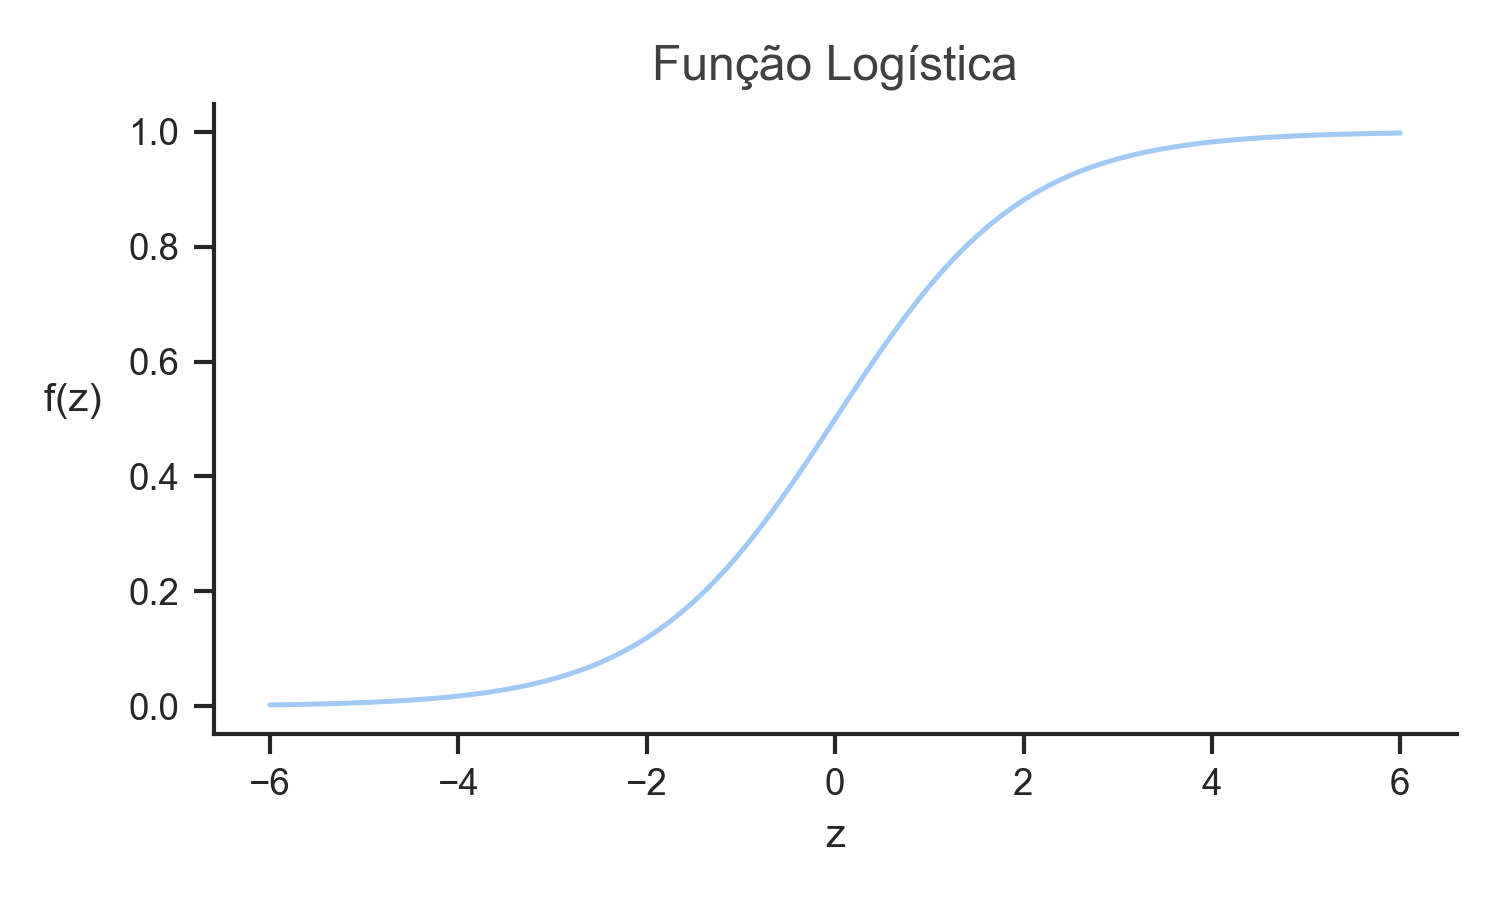
\includegraphics[scale=0.7]{USPSC-img/funcao-logistica.png}
    \begin{center}
        Fonte: Autor (2023).
    \end{center}
\end{figure}

\subsection{Máquinas de Vetores de Suporte}

As Máquinas de Vetores de Suporte, ou \textit{Support Vector Machines} (SVM), são um método de aprendizado supervisionado que busca encontrar o hiperplano de separação que maximiza a margem entre as classes. Elas são usadas em problemas de classificação para encontrar a melhor fronteira de decisão entre as classes, permitindo sobreposição entre elas, mas minimizando essa sobreposição. As SVMs são particularmente úteis em problemas de classificação com muitas características, onde outras técnicas podem sofrer de sobreajuste, o que as torna robustas em relação a ruídos e \textit{outliers} \cite{trevorHastie}.

As SVMs podem lidar com conjuntos de dados não lineares por meio do uso de \textit{kernels}, que mapeiam os dados para um espaço de maior dimensão onde eles podem ser separados linearmente. Na \autoref{img:kernelsvm}, é apresentado um exemplo de um espaço de características que foi transformado.

\begin{figure}[htb]
	\centering
	\caption{\label{img:kernelsvm}Exemplo de transformação utilizando \textit{kernel}: Convertendo um problema de classificação não linear em um problema de classificação linear em uma dimensão superior.}
	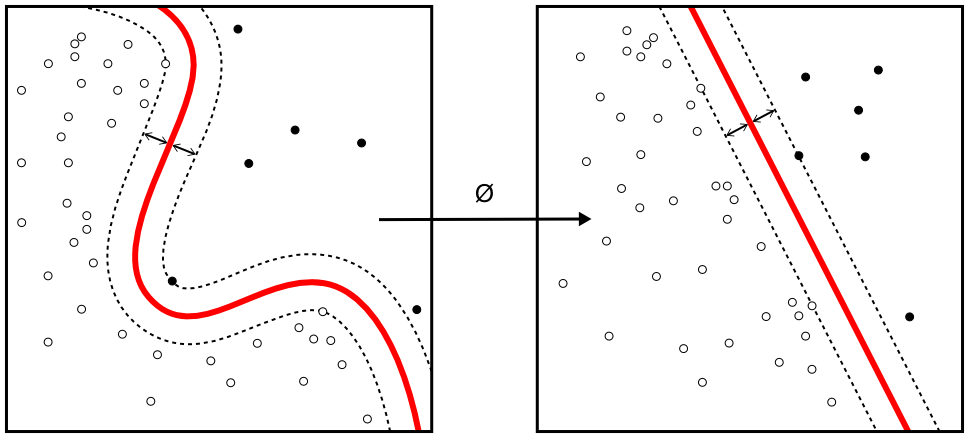
\includegraphics[scale=0.5]{USPSC-img/Kernel_Machine.png}
	\begin{center}
		Fonte: \cite{wiki}.
	\end{center}
\end{figure}

Embora as SVMs sejam amplamente utilizadas e tenham várias vantagens, também apresentam algumas desvantagens. Uma das principais desvantagens das SVMs é a necessidade de ajuste cuidadoso dos parâmetros do modelo, como o parâmetro de regularização e a escolha do \textit{kernel}, o que pode ser uma tarefa desafiadora e exigir conhecimento especializado. Além disso, as SVMs podem ser computacionalmente intensivas, especialmente em conjuntos de dados muito grandes, o que pode tornar seu treinamento demorado. Outra limitação das SVMs é a dificuldade em lidar com conjuntos de dados com muitas classes, uma vez que a abordagem de um-contra-um para problemas multiclasse pode levar a um grande número de classificadores binários \cite{trevorHastie}.

\subsection{Florestas Aleatórias e \textit{Gradient Boosted Trees}}

As Florestas Aleatórias (do inglês \textit{Random Forests}) e \textit{Gradient Boosted Trees} são exemplos de comitês (\textit{ensembles}) de algoritmos de aprendizado de máquina. Resumidamente, o método consiste na construção de múltiplas árvores de decisão em subespaços aleatórios do espaço de características, utilizando amostras aleatórias dos dados de treinamento e subconjuntos aleatórios das características disponíveis. Cada árvore de decisão é capaz de generalizar sua classificação de forma única, e a combinação das previsões de todas as árvores resulta em uma melhoria monotônica na precisão da classificação \cite{RandomForests}. Estudos recentes têm indicado que a aplicação desses algoritmos tem apresentado desempenho superior na previsão em comparação com outros métodos de aprendizado de máquina \cite{geron2022hands, Raschka}. Na \autoref{img:rfexample}, é ilustrada a construção de três árvores de decisão para um problema de classificação, construídas pelo algoritmo \textit{Random Forest}.

\begin{figure}
	\centering
	\caption{\label{img:rfexample}Ilustração do algoritmo \textit{Random Forest}.}
	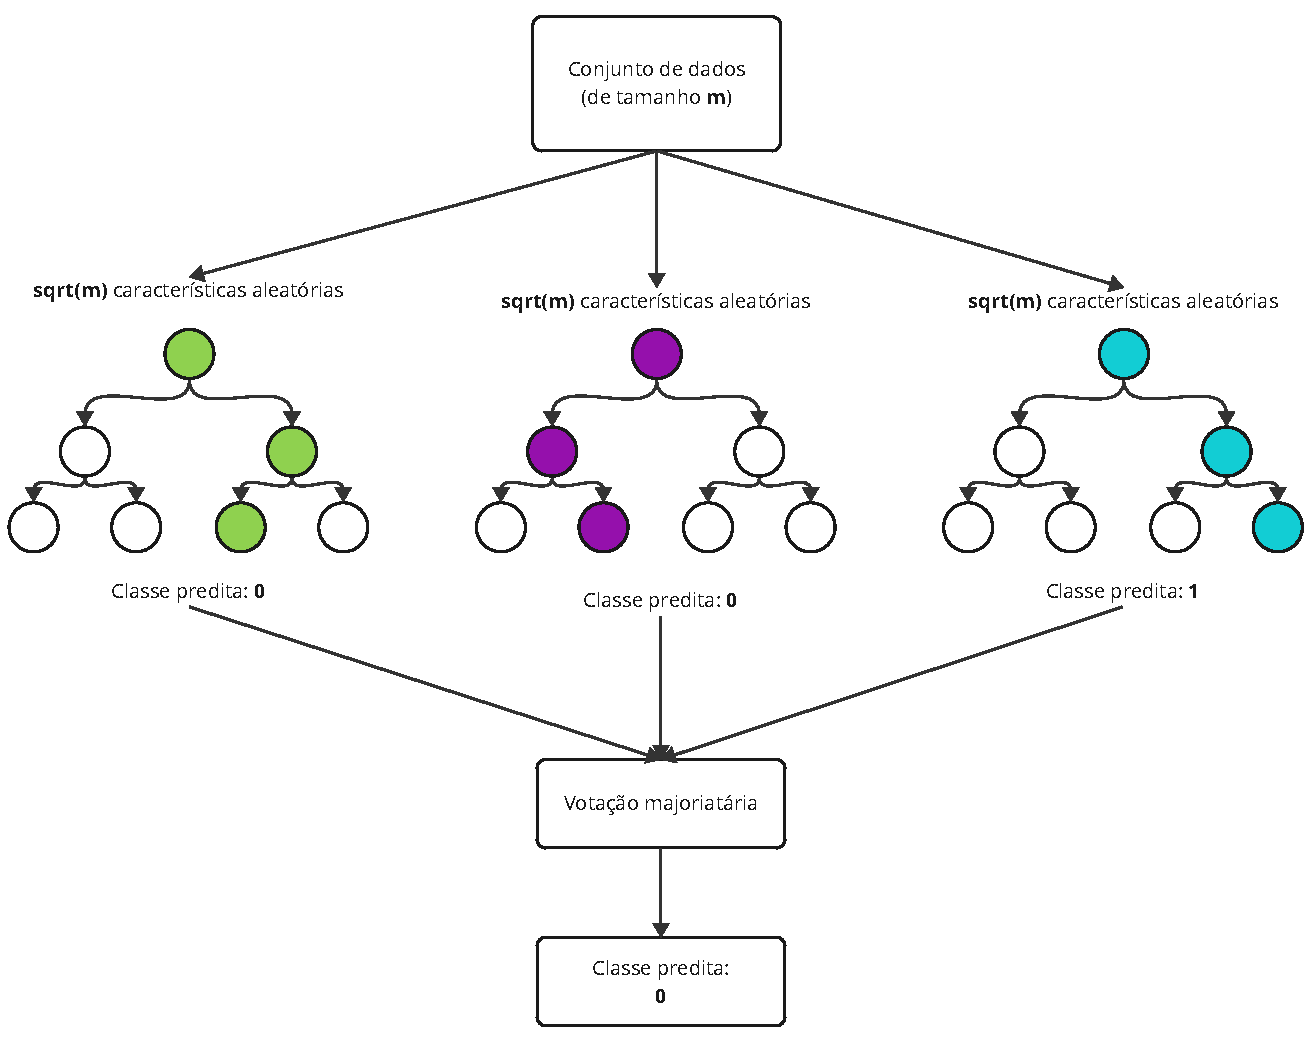
\includegraphics[scale=0.7]{USPSC-img/random_forest_example.pdf}
	\begin{center}
		Fonte: Adaptado de \citeonline{mlaplicadosaude}.
	\end{center}
\end{figure}

Com o objetivo de melhorar a precisão das previsões das árvores de decisão, o algoritmo \textit{Gradient Boosted Trees} \cite{friedman2000} utiliza a estratégia de \textit{boosting}. Em termos mais detalhados, o processo de \textit{boosting} geralmente começa com um modelo base simples, como uma árvore de decisão rasa. Este modelo é treinado no conjunto de dados e usado para fazer previsões. Em seguida, os exemplos que foram classificados incorretamente ou para os quais as previsões tiveram grandes erros são ponderados mais fortemente no próximo modelo a ser treinado. Este próximo modelo é treinado para se concentrar nos exemplos que foram mal classificados pelo modelo anterior, e o processo é repetido \cite{friedman2000}.

Ainda segundo \citeonline{friedman2000}, a técnica de \textit{Gradient Boosting} proposta pelo autor permitiu avanços importantes na capacidade de lidar com problemas complexos de previsão e classificação. Essa abordagem influenciou diretamente o desenvolvimento de algoritmos populares, como \textit{XGBoost} e \textit{LightGBM}, que são amplamente utilizados em competições de ciência de dados e em aplicações do mundo real devido à sua eficácia e desempenho.

\section{Inteligência Artificial Explicável}

A Inteligência Artificial Explicável refere-se à capacidade de compreender e explicar as decisões e previsões dos modelos de inteligência artificial. A explicabilidade é crucial para estabelecer a confiança do usuário, fornecer insights sobre como melhorar o modelo e compreender o processo que está sendo modelado. A capacidade de interpretar corretamente a saída de um modelo de previsão é extremamente importante, especialmente em contextos nos quais modelos complexos e de alto desempenho são utilizados \cite{Shap2017}. Nesta seção, será fornecida uma breve exposição do método de XAI aplicado neste trabalho, o \textit{SHapley Additive exPlanations} (SHAP).

\subsection{\textit{SHapley Additive exPlanations} (SHAP)}\label{sec:shap}

O SHAP \cite{Shap2017} unifica seis métodos existentes de interpretação de predições: LIME, DeepLIFT, Layer-wise Relevance Propagation (LRP), Shapley sampling values, SmoothGrad e Integrated Gradients.

O \textit{Local Interpretable Model-Agnostic Explanations} (LIME) \cite{Lime2016} é um método que explica as previsões de um modelo complexo construindo um modelo localmente interpretável em torno da previsão. O DeepLIFT \cite{Deeplift} compara a ativação de cada variável na previsão atual com a ativação média da variável em todas as previsões. O LRP \cite{LRP2015} atribui a importância de cada variável para uma previsão propagando a relevância da saída do modelo de volta para as entradas. O Shapley sampling values \cite{Strumbelj2014} amostra aleatoriamente subconjuntos de variáveis e calcula a contribuição média de cada variável para a previsão. O SmoothGrad \cite{SmoothGrad} suaviza as entradas do modelo para reduzir o ruído e, em seguida, calcula a importância de cada variável para uma previsão. O Integrated Gradients \cite{IntegratedGradients} integra a contribuição de cada variável para uma previsão ao longo de um caminho suave entre a entrada atual e uma entrada de referência.

O SHAP unifica esses métodos por meio da introdução do conceito de \q{modelo de explicação}, que representa uma aproximação interpretável do modelo original. Além disso, fornece resultados teóricos que asseguram a existência de uma solução única na classe de métodos aditivos, atendendo a um conjunto de propriedades desejáveis, incluindo consistência, localidade e completude. O SHAP propõe uma nova medida de importância de variáveis chamada \textit{SHAP value}, a única medida aditiva que satisfaz essas propriedades. Esses valores, conforme demonstrado pelo SHAP, estão alinhados com a intuição humana e são eficazes na discriminação entre classes de saída do modelo \cite{Shap2017}.

\section{Trabalhos de classificação na área médica}\label{sec-context}

A utilização de algoritmos de aprendizado de máquina para análises preditivas é uma tarefa que envolve uma série de etapas que vão desde  a preparação dos dados, até o lançamento e monitoramento da solução \cite{geron2022hands}. O trabalho de \citeonline{SantosHellenGeremiasdos2019Mlpa} se propõe a exemplificar as etapas envolvidas na utilização desses algoritmos para análises preditivas em saúde, com um exemplo de aplicação para predizer óbito em idosos de São Paulo. A metodologia empregada envolveu a utilização de diferentes algoritmos de aprendizado de máquina para treinar modelos preditivos a partir de dados do estudo SABE, e a avaliação desses modelos em termos de acurácia, sensibilidade e especificidade. Os resultados mostraram que os modelos tiveram desempenho razoável na predição de óbito em idosos, com destaque para o algoritmo Random Forest. No entanto, os autores ressaltam que a amostra utilizada foi relativamente pequena e que a performance dos modelos pode ser melhorada com mais dados e refinamento dos algoritmos.

O trabalho de \citeonline{LORETO2020103636} aborda a predição de reinternações em UTI usando algoritmos de classificação. A proposta é investigar se as características basais e informações coletadas no momento da admissão do paciente podem possibilitar previsões precisas de reinternação na UTI. A metodologia empregada envolveu a análise de um conjunto de dados de 11.805 pacientes adultos de três UTIs em um hospital universitário brasileiro, com a exclusão de pacientes falecidos durante a primeira admissão na UTI. Foram testados oito algoritmos de classificação e avaliados com base em seis métricas. Os resultados mostraram que as características do paciente registradas na admissão na UTI foram capazes de prever o risco de reinternação, superando modelos anteriores que utilizavam apenas dados disponíveis na alta da UTI.

\citeonline{WANG2021351} apresentam um estudo sobre a estimativa da probabilidade de reinternação à UTI para pacientes transferidos da UTI para a enfermaria geral, abordando os desafios de dados desbalanceados e esparsos. A pesquisa visa melhorar a gestão médica e reduzir as taxas de reinternação à UTI, levando a melhores resultados para os pacientes e redução de custos de saúde. A metodologia empregada inclui a análise de valores ausentes, o teste de razão de verossimilhança e a utilização de um modelo de floresta aleatória com decaimento de peso. Os resultados mostram que o modelo proposto supera outros métodos tradicionais em sete indicadores de desempenho diferentes.

O artigo de \citeonline{Stiglic2014} propõe uma abordagem para a classificação de reinternações pediátricas usando modelos de diferentes hospitais, permitindo alta performance e compreensibilidade dos resultados. A metodologia empregada é baseada em \textit{deep learning} e \textit{stacked generalization}, e foi avaliada usando dados de 54 hospitais na Califórnia para demonstrar as possibilidades de implantação em larga escala. Os resultados mostraram melhorias significativas no desempenho de classificação e interpretabilidade dos resultados.

O trabalho de \citeonline{CDCWound} tem como objetivo avaliar se a classificação de feridas do \textit{Centers for Disease Control and Prevention} (CDC) pode ser usada como um indicador de risco para reinternação hospitalar em 30 dias após a cirurgia. A metodologia empregada foi uma revisão retrospectiva de pacientes submetidos a cirurgias eletivas em um hospital universitário. Os resultados mostraram que a classificação de feridas do CDC foi um preditor significativo de reinternação hospitalar em 30 dias após a cirurgia. Os autores concluem que a classificação de feridas do CDC pode ser uma ferramenta útil para identificar pacientes com maior risco de reinternação hospitalar após a cirurgia.

\citeonline{fernandes2021multipurpose} apresentam uma abordagem multipropósito de aprendizado de máquina para prever o prognóstico negativo da COVID-19 em São Paulo, Brasil. O trabalho envolveu o treinamento de cinco algoritmos de aprendizado de máquina com dados estruturados de pacientes com COVID-19, utilizando técnicas de validação cruzada e otimização bayesiana. O objetivo era prever o risco de desenvolver condições críticas em pacientes com COVID-19. Os resultados mostraram que a abordagem proposta teve um desempenho satisfatório na previsão do prognóstico negativo da COVID-19, o que pode ajudar na tomada de decisões clínicas e na alocação efetiva de recursos de saúde.

O trabalho de \citeonline{genesdisease} propõe uma metodologia baseada em aprendizado de máquina para identificar genes relacionados a doenças complexas. O modelo de aprendizado de máquina proposto utiliza uma matriz de similaridade funcional entre genes para prever doenças genéticas complexas. Essa matriz é construída a partir de medidas de similaridade entre genes, como perfis de expressão gênica, redes de interação proteína-proteína e Gene Ontology. Em seguida, um classificador de aprendizado de máquina é treinado com essa matriz para identificar genes relevantes para a doença em questão. O modelo proposto foi avaliado em relação à sua capacidade de identificar genes relacionados ao Transtorno do Espectro Autista e mostrou melhorias significativas em relação a outros métodos de identificação de genes. Foi desenvolvido um fluxo de trabalho automatizado para tornar a metodologia acessível a pesquisadores sem conhecimento extenso em programação e aprendizado de máquina.

\citeonline{rosa_galdamez_souza_melo_villarinho_leal_2023} apresentam um estudo que utiliza técnicas de aprendizado de máquina para classificar fatores que influenciam a ocorrência de dermatites ocupacionais. A metodologia empregada envolveu a avaliação de diferentes algoritmos de aprendizado de máquina, a comparação dos resultados obtidos por cada técnica e a identificação dos fatores mais influentes na ocorrência da lesão ocupacional. Os resultados indicaram que todas as técnicas apresentaram acuracidade entre 55\% e 69,4\%, sensitividade entre 49,1\% e 80,7\% e especificidade entre 50\% e 66,7\%. Os fatores mais influentes identificados foram a exposição a produtos químicos, o uso de equipamentos de proteção individual inadequados e a falta de treinamento adequado.

\section{Técnicas de explicação aplicadas a trabalhos de classificação na área médica}\label{sec-context}

A explicabilidade já foi identificada como um fator chave para a adoção de sistemas de IA numa vasta gama de contextos \cite{doshivelez2017rigorous, lipton2017mythos, ribeiro2016modelagnostic}. No estudo conduzido por \citeonline{Abououf2023}, é apresentado um sistema de monitoramento de saúde que utiliza inteligência artificial para detectar e classificar eventos e anomalias médicas. A metodologia empregada envolve a utilização de um modelo de detecção de anomalias e eventos, um modelo de classificação e uma técnica de explicabilidade chamada \textit{KernelSHAP}. O sistema foi avaliado em um conjunto de dados de pacientes e obteve resultados promissores na detecção e classificação de eventos e anomalias médicas. Além disso, a técnica de explicabilidade permitiu que os médicos entendessem melhor as decisões tomadas pelo sistema de inteligência artificial.

Com o uso de técnicas de aprendizado profundo e transferência de aprendizado para detectar a COVID-19 a partir de radiografias de tórax, o estudo de \citeonline{BRUNESE2020105608} utiliza as camadas de ativação da rede, ou seja, as áreas da radiografia de tórax que o modelo considerou para gerar a predição, para fornecer explicabilidade sobre a predição. Ainda segundo os autores, isso pode representar uma sugestão para o radiologista localizar imediatamente as áreas da radiografia de tórax que podem ser de interesse. Os resultados mostraram que o modelo proposto alcançou uma acurácia de 98,08\% na detecção de COVID-19 em radiografias de tórax. O estudo também sugere que essa tecnologia pode ser usada como uma ferramenta de triagem para ajudar no diagnóstico da COVID-19 em configurações clínicas do mundo real.

No trabalho de \citeonline{KIM2022103677} foi desenvolvida uma técnica de previsão de mortalidade relacionada ao calor em uma unidade espacial detalhada dentro de uma cidade, utilizando um modelo baseado em floresta aleatória e a técnica de explicação SHAP. A metodologia empregada incluiu a coleta de dados meteorológicos, demográficos e socioeconômicos, pré-processamento de dados, divisão em conjuntos de treinamento e teste, construção do modelo, otimização de hiperparâmetros, avaliação de desempenho e interpretação dos resultados. Os resultados mostraram que o modelo proposto é capaz de prever com precisão a mortalidade relacionada ao calor em uma área específica da cidade de Daegu, na Coreia do Sul. A técnica SHAP permitiu uma interpretação global e local dos resultados, identificando as variáveis mais importantes para a previsão.

Também utilizando modelos SHAP, o trabalho de \citeonline{healthcare11070929} utiliza técnicas para prever a fertilidade masculina, com o intuito de melhorar a transparência, responsabilidade e explicabilidade de sete modelos de IA padrão da indústria. A metodologia empregada consistiu em coletar dados de pacientes com problemas de fertilidade masculina e aplicar os modelos de IA para prever a fertilidade. Em seguida, foram utilizadas técnicas de amostragem e validação cruzada para avaliar a robustez e estabilidade de cada modelo. Por fim, a técnica de XAI foi utilizada para explicar o desempenho de cada modelo e os resultados mostraram que o SHAP foi capaz de interpretar as previsões dos sistemas de IA e fornecer explicações claras e compreensíveis para os usuários.